\documentclass[tikz]{standalone}

\usepackage{tikz}
\usepackage{xcolor}
\usepackage{pgfplots}
\usepackage{../tikzviolinplots}
%\usepgfplotslibrary{external}
%\tikzexternalize
\usepackage{siunitx}
\usepackage{fontspec}
\pgfplotsset{compat=1.18}
\setmainfont{Source Serif 4}[
    Renderer = OpenType,
    SizeFeatures    = {%
        {Size={-9},Font=* Caption},
        {Size={9-13},Font=*},
        {Size={14-24},Font=* Subhead},
        {Size={24-},Font=* Display}
    },
    ItalicFeatures = {%
    SizeFeatures    = {%
            {Size={-9},Font=* Caption Italic},
            {Size={9-13},Font=* Italic},
            {Size={14-24},Font=* Subhead Italic},
            {Size={24-},Font=* Display Italic}
    },
    },
    BoldFeatures = {%
    SizeFeatures    = {%
            {Size={-9},Font=* Caption Semibold},
            {Size={9-13},Font=* Semibold},
            {Size={14-24},Font=* Subhead Semibold},
            {Size={24-},Font=* Display Semibold}
    },
    },
    BoldItalicFeatures = {%
    SizeFeatures    = {%
            {Size={-9},Font=* Caption Semibold Italic},
            {Size={9-13},Font=* Semibold Italic},
            {Size={14-24},Font=* Subhead Semibold Italic},
            {Size={24-},Font=* Display Semibold Italic}
    },
    },
    Numbers         = OldStyle,
]

\usetikzlibrary{shapes,arrows,positioning,backgrounds,calc,intersections,calc,svg.path,fit,fpu}
\definecolor{ugent-re}{RGB}{220, 78, 40}        % vermilion			/ vermiljoen
\definecolor{ugent-we}{RGB}{45, 140, 168}       % no match

\begin{document}
\begin{filecontents}[overwrite]{violin-small.dat}
    A,B,C,D,E
    0.0001,0.0001,0.0001,0.0001,0.0001
    0.0001,0.0001,0.0001,0.0001,0.0001
    0.0001,0.0001,0.0001,0.0001,0.0001
    0.0001,0.0001,0.0001,0.0001,0.0001
    0.0001,0.0001,0.0001,0.0001,0.0001
    0.0001,0.0001,0.0001,0.0001,0.0001
    0.0001,0.0001,0.0001,0.0001,0.0001
    0.0001,0.0001,0.0001,0.0001,0.0001
    0.0001,0.0001,0.0001,0.0001,0.0001
    0.0001,0.0001,0.0001,0.0001,0.0001
    0.0001,0.0001,0.0001,0.0001,0.0001
    0.00016,0.00019,0.0002,0.00019,0.0002
    -0.00352,-0.00181,-0.00063,0.00081,0.00103
    0.0001,0.0001,0.0001,0.0001,0.0001
    2e-05,0.00012,0.00014,0.00014,0.00014
    0.0001,0.0001,0.0001,0.0001,0.0001
    0.0001,0.0001,0.0001,0.0001,0.0001
    0.0001,0.0001,0.0001,0.0001,0.0001
    0.0001,0.0001,0.0001,0.0001,0.0001
    0.0001,0.0001,0.0001,0.0001,0.0001
    0.0001,0.0001,0.0001,0.0001,0.0001
    -0.00115,0.00065,0.00156,0.0026,0.00233
    0.0001,0.0001,0.0001,0.0001,0.0001
    0.0001,0.0001,0.0001,0.0001,0.0001
    0.0001,0.0001,0.0001,0.0001,0.0001
    0.0001,0.0001,0.0001,0.0001,0.0001
    0.0001,0.0001,0.0001,0.0001,0.0001
    -0.00041,-0.00016,-4e-05,-0.0,0.00015
    0.00013,0.00014,0.00015,0.00015,0.00017
    -0.00613,-0.00166,0.00098,0.00295,0.00145
    0.0001,0.0001,0.0001,0.0001,0.0001
    0.0001,0.0001,0.0001,0.0001,0.0001
    0.0001,0.0001,0.0001,0.0001,0.0001
    0.0001,0.0001,0.0001,0.0001,0.0001
    0.0001,0.0001,0.0001,0.0001,0.0001
    0.00012,0.00359,0.00568,0.00757,0.00656
    0.0001,0.0001,0.0001,0.0001,0.0001
    0.0001,0.0001,0.0001,0.0001,0.0001
    0.0001,0.0001,0.0001,0.0001,0.0001
    -6.15727,-6.66999,-6.81233,-7.39451,-10.57109
    0.0001,0.0001,0.0001,0.0001,0.0001
    0.0001,0.0001,0.0001,0.0001,0.0001
    -4e-05,0.0001,0.00011,9e-05,0.00025
    0.0001,0.00177,0.00302,0.00432,0.00447
    0.0001,0.0001,0.0001,0.0001,0.0001
    0.0001,0.0001,0.0001,0.0001,0.0001
    0.0001,0.0001,0.0001,0.0001,0.0001
    0.0001,0.0001,0.0001,0.0001,0.0001
    9e-05,0.00157,0.00263,0.00388,0.00375
    0.00018,0.00021,0.00031,0.00034,0.00042
    0.0001,0.0001,0.0001,0.0001,0.0001
    0.0001,0.0001,0.0001,0.0001,0.0001
    0.0001,0.0001,0.0001,0.0001,0.0001
    0.0001,0.0001,0.0001,0.0001,0.0001
    0.0001,0.0001,0.0001,0.0001,0.0001
    0.0001,0.0001,0.0001,0.0001,0.0001
    0.0001,0.0001,0.0001,0.0001,0.0001
    0.0001,0.0001,0.0001,0.0001,0.0001
    0.0001,0.0001,0.0001,0.0001,0.0001
    1e-05,0.00134,0.00252,0.00359,0.00352
    0.0001,0.0001,0.0001,0.0001,0.0001
    0.0001,0.00153,0.00276,0.0038,0.00373
    0.0001,0.00148,0.00258,0.00367,0.00372
    0.0001,0.0001,0.0001,0.0001,0.0001
    0.0001,0.0001,0.0001,0.0001,0.0001
    -0.0001,-6e-05,-3e-05,-3e-05,2e-05
    -0.00042,-0.00042,-0.00042,-0.00042,-0.00042
    -0.01045,-0.00443,-0.00032,0.0033,0.00359
    0.0001,0.0001,0.0001,0.0001,0.0001
    9e-05,0.00331,0.0059,0.00747,0.00609
    0.0001,0.0001,0.0001,0.0001,0.0001
    0.0001,0.0001,0.0001,0.0001,0.0001
    -3.24683,-4.8678,-5.30228,-6.20039,-9.73571
    0.0001,0.0001,0.0001,0.0001,0.0001
    0.0001,0.0001,0.0001,0.0001,0.0001
\end{filecontents}
\begin{tikzpicture}
    \pgfplotsset{height=5cm,width=6cm}
    \pgfkeys{/pgfplots/yticklabel={\addfontfeature{Numbers={Lining}}\qty[round-mode=places, round-precision=0]{\tick}{\mega{}}},}
    \violinsetoptions[
        scaled,
        averages,
    ]{
        xmin=0.3,xmax=6.2,
        ymin=-13,ymax=4,
        xlabel style={
            yshift = {-3*height("a")}
        },
        ymajorgrids=true,
        ytick distance=3,
        ylabel={№ of blocks}
    }
    \violinplot[%
        index=A,
        relative position=1,
        label={30},
        samples=100,
        average mark=*,
        average fill=black,
        average fill opacity=1.0,
        average size=1pt,
        color=ugent-we,
    ]{violin-small.dat}
    \violinplot[%
        index=B,
        relative position=2.2,
        label={60},
        samples=100,
        average mark=*,
        average fill=black,
        average fill opacity=1.0,
        average size=1pt,
        color=ugent-we,
    ]{violin-small.dat}
    \violinplot[%
        index=C,
        relative position=3.3,
        label={90},
        samples=100,
        average mark=*,
        average fill=black,
        average fill opacity=1.0,
        average size=1pt,
        color=ugent-we,
    ]{violin-small.dat}
    \violinplot[%
        index=D,
        relative position=4.4,
        label={120},
        samples=100,
        average mark=*,
        average fill=black,
        average fill opacity=1.0,
        average size=1pt,
        color=ugent-we,
    ]{violin-small.dat}
    %! parser = off
    \pgfkeys{
        /pgfplots/xticklabels={\addfontfeature{Numbers={OldStyle,Proportional}}\textsc{asap}},
        /pgfplots/xlabel={Execution models (\textsc{em-})},
    };
    %! parser = on
    \violinplot[%
        index=E,
        relative position=5.5,
        samples=100,
        average mark=*,
        average fill=black,
        average fill opacity=1.0,
        average size=1pt,
    ]{violin-small.dat}
\end{tikzpicture}
\end{document}
